\documentclass[journal,12pt,twocolumn]{IEEEtran}

\usepackage{graphicx}
\usepackage{setspace}
\usepackage{gensymb}
\singlespacing
\usepackage[cmex10]{amsmath}
\usepackage{amssymb}
\usepackage{xurl}
\usepackage{tabularx}
\usepackage{amsthm}
\usepackage{comment}
\usepackage{mathrsfs}
\usepackage{txfonts}
\usepackage{stfloats}
\usepackage{bm}
\usepackage{cite}
\usepackage{cases}
\usepackage{subfig}
\usepackage{arydshln}
\usepackage{longtable}
\usepackage{multirow}

\usepackage{enumitem}
\usepackage{mathtools}
\usepackage{steinmetz}
\usepackage{tikz}
\usepackage{circuitikz}
\usepackage{verbatim}
\usepackage{tfrupee}
\usepackage[breaklinks=true]{hyperref}
\usepackage{graphicx}
\usepackage{tkz-euclide}
\usetikzlibrary{automata, positioning}
\usetikzlibrary{calc,math}
\usepackage{listings}
    \usepackage{color}                                            %%
    \usepackage{array}                                            %%
    \usepackage{longtable}                                        %%
    \usepackage{calc}                                             %%
    \usepackage{multirow}                                         %%
    \usepackage{hhline}                                           %%
    \usepackage{ifthen}                                           %%
    \usepackage{lscape}     
\usepackage{multicol}
\usepackage{chngcntr}
\usepackage{blkarray}

\DeclareMathOperator*{\Res}{Res}

\renewcommand\thesection{\arabic{section}}
\renewcommand\thesubsection{\thesection.\arabic{subsection}}
\renewcommand\thesubsubsection{\thesubsection.\arabic{subsubsection}}

\renewcommand\thesectiondis{\arabic{section}}
\renewcommand\thesubsectiondis{\thesectiondis.\arabic{subsection}}
\renewcommand\thesubsubsectiondis{\thesubsectiondis.\arabic{subsubsection}}


\hyphenation{op-tical net-works semi-conduc-tor}
\def\inputGnumericTable{}                                 %%

\lstset{
%language=C,
frame=single, 
breaklines=true,
columns=fullflexible
}
\begin{document}


\newtheorem{theorem}{Theorem}[section]
\newtheorem{problem}{Problem}
\newtheorem{proposition}{Proposition}[section]
\newtheorem{lemma}{Lemma}[section]
\newtheorem{corollary}[theorem]{Corollary}
\newtheorem{example}{Example}[section]
\newtheorem{definition}[problem]{Definition}

\newcommand{\BEQA}{\begin{eqnarray}}
\newcommand{\EEQA}{\end{eqnarray}}
\newcommand{\define}{\stackrel{\triangle}{=}}
\bibliographystyle{IEEEtran}
\raggedbottom
\setlength{\parindent}{0pt}
\providecommand{\mbf}{\mathbf}
\providecommand{\pr}[1]{\ensuremath{\Pr\left(#1\right)}}
\providecommand{\qfunc}[1]{\ensuremath{Q\left(#1\right)}}
\providecommand{\sbrak}[1]{\ensuremath{{}\left[#1\right]}}
\providecommand{\lsbrak}[1]{\ensuremath{{}\left[#1\right.}}
\providecommand{\rsbrak}[1]{\ensuremath{{}\left.#1\right]}}
\providecommand{\brak}[1]{\ensuremath{\left(#1\right)}}
\providecommand{\lbrak}[1]{\ensuremath{\left(#1\right.}}
\providecommand{\rbrak}[1]{\ensuremath{\left.#1\right)}}
\providecommand{\cbrak}[1]{\ensuremath{\left\{#1\right\}}}
\providecommand{\lcbrak}[1]{\ensuremath{\left\{#1\right.}}
\providecommand{\rcbrak}[1]{\ensuremath{\left.#1\right\}}}
\theoremstyle{remark}
\newtheorem{rem}{Remark}
\newcommand{\sgn}{\mathop{\mathrm{sgn}}}
\providecommand{\abs}[1]{\vert#1\vert}
\providecommand{\res}[1]{\Res\displaylimits_{#1}} 
\providecommand{\norm}[1]{\lVert#1\rVert}
%\providecommand{\norm}[1]{\lVert#1\rVert}
\providecommand{\mtx}[1]{\mathbf{#1}}
\providecommand{\mean}[1]{E[ #1 ]}
\providecommand{\fourier}{\overset{\mathcal{F}}{ \rightleftharpoons}}
%\providecommand{\hilbert}{\overset{\mathcal{H}}{ \rightleftharpoons}}
\providecommand{\system}{\overset{\mathcal{H}}{ \longleftrightarrow}}
	%\newcommand{\solution}[2]{\textbf{Solution:}{#1}}
\newcommand{\solution}{\noindent \textbf{Solution: }}
\newcommand{\cosec}{\,\text{cosec}\,}
\providecommand{\dec}[2]{\ensuremath{\overset{#1}{\underset{#2}{\gtrless}}}}
\newcommand{\myvec}[1]{\ensuremath{\begin{pmatrix}#1\end{pmatrix}}}
\newcommand{\mydet}[1]{\ensuremath{\begin{vmatrix}#1\end{vmatrix}}}
\newcommand*{\permcomb}[4][0mu]{{{}^{#3}\mkern#1#2_{#4}}}
\newcommand*{\perm}[1][-3mu]{\permcomb[#1]{P}}
\newcommand*{\comb}[1][-1mu]{\permcomb[#1]{C}}
\numberwithin{equation}{subsection}
\makeatletter
\@addtoreset{figure}{problem}
\makeatother
\let\StandardTheFigure\thefigure
\let\vec\mathbf
\renewcommand{\thefigure}{\theproblem}
\def\putbox#1#2#3{\makebox[0in][l]{\makebox[#1][l]{}\raisebox{\baselineskip}[0in][0in]{\raisebox{#2}[0in][0in]{#3}}}}
     \def\rightbox#1{\makebox[0in][r]{#1}}
     \def\centbox#1{\makebox[0in]{#1}}
     \def\topbox#1{\raisebox{-\baselineskip}[0in][0in]{#1}}
     \def\midbox#1{\raisebox{-0.5\baselineskip}[0in][0in]{#1}}
\vspace{3cm}
\title{\textbf{LINEAR SYSTEMS AND SIGNAL PROCESSING \\ GATE ASSIGNMENT 1}}
\author{GANJI VARSHITHA - AI20BTECH11009}
\maketitle
\newpage
\bigskip
\renewcommand{\thefigure}{\arabic{figure}}
\renewcommand{\thetable}{\arabic{table}}
Download latex codes from 
%
\begin{lstlisting}
https://github.com/VARSHITHAGANJI/EE3900_GATE_ASSIGNMENTS/blob/main/GATE_ASSIGNMENT1/GATE_ASSIGNMENT1.tex
\end{lstlisting}
\section*{QUESTION}
\textbf{GATE EC-2019 Question 28}
\\
Consider a six-point decimation-in-time Fast Fourier Transform \brak{\text{FFT}} algorithm, for which the signal-flow graph corresponding to X\sbrak{1} is shown in the figure. Let $W_{6}=\text{exp\brak{-\frac{j2\pi}{6}}}$. In the figure, what should be the values of the coefficients $a_{1}, a_{2}, a_{3}$ in terms of $W_{6}$ so that X\sbrak{1} is obtained correctly?
\begin{figure}[h]
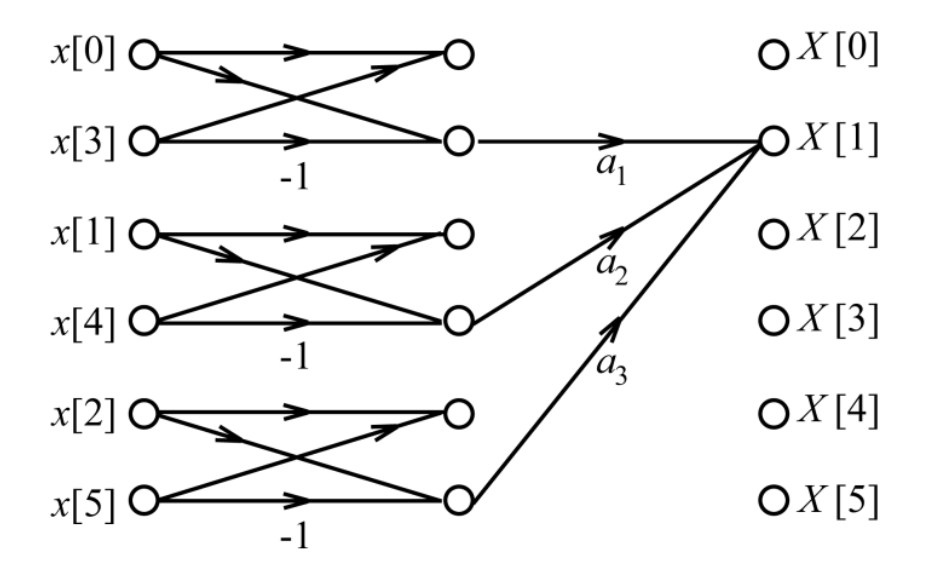
\includegraphics[width=5cm, height=4cm]{gateq1}
\centering
\end{figure}
\begin{enumerate}
   \item  $a_{1}=-1, a_{2}=W_{6}, a_{3}=W_{6}^{2}$ 
   \item  $a_{1}=1, a_{2}=W_{6}^{2}, a_{3}=W_{6}$ 
   \item  $a_{1}=1, a_{2}=W_{6}, a_{3}=W_{6}^{2}$ 
   \item  $a_{1}=-1, a_{2}=W_{6}^{2}, a_{3}=W_{6}$ 
   
\end{enumerate}
\section*{SOLUTION}
Considering six-point DFT, we have 

\begin{align}
\label{eq:1}
\myvec{X\sbrak{0}\\X\sbrak{1}\\X\sbrak{2}\\X\sbrak{3}\\X\sbrak{4}\\X\sbrak{5}} = \myvec{W_{6}^{0}&W_{6}^{1}&W_{6}^{2}&W_{6}^{3}&W_{6}^{4}&W_{6}^{5}\\W_{6}^{0}&W_{6}^{1}&W_{6}^{2}&W_{6}^{3}&W_{6}^{4}&W_{6}^{5}\\W_{6}^{0}&W_{6}^{1}&W_{6}^{2}&W_{6}^{3}&W_{6}^{4}&W_{6}^{5}\\W_{6}^{0}&W_{6}^{1}&W_{6}^{2}&W_{6}^{3}&W_{6}^{4}&W_{6}^{5}\\W_{6}^{0}&W_{6}^{1}&W_{6}^{2}&W_{6}^{3}&W_{6}^{4}&W_{6}^{5}\\W_{6}^{0}&W_{6}^{1}&W_{6}^{2}&W_{6}^{3}&W_{6}^{4}&W_{6}^{5}}\myvec{x\sbrak{0}\\x\sbrak{1}\\x\sbrak{2}\\x\sbrak{3}\\x\sbrak{4}\\x\sbrak{5}}
\end{align}
where twiddler factor $W_{6} = \text{exp}\brak{-\frac{j2\pi}{6}}$.

By symmetric property of twiddler factor 
\begin{center}
$W_{N}^{k+\frac{N}{2}} = -W_{N}^{k}$ , where N=6.
\end{center}
Putting k = 0, 1, 2 , we get 
\begin{align}
\label{eq:2}
W_{6}^{3}={}&-W_{6}^{0}\\
\label{eq:3}
W_{6}^{4}={}&-W_{6}^{1}\\
\label{eq:4}
W_{6}^{5}={}&-W_{6}^{2}
\end{align}
respectively.\\
Obtaining X\sbrak{1} by substituting \eqref{eq:2}, \eqref{eq:3}, \eqref{eq:4} in \eqref{eq:1}, we get,
\begin{align}
\label{eq:5}
X\sbrak{1}={}&\myvec{W_{6}^{0}&W_{6}^{1}&W_{6}^{2}&-W_{6}^{0}&-W_{6}^{1}&-W_{6}^{2}}\myvec{x\sbrak{0}\\x\sbrak{1}\\x\sbrak{2}\\x\sbrak{3}\\x\sbrak{4}\\x\sbrak{5}}
\end{align}
\begin{align}
\label{eq:6}
={}&\myvec{W_{6}^{0}&W_{6}^{1}&W_{6}^{2}}\myvec{1 & 0 & 0 & -1 & 0 & 0\\0 & 1 & 0 & 0 & -1 & 0\\0 & 0 & 1 & 0 & 0 & -1}\myvec{x\sbrak{0}\\x\sbrak{1}\\x\sbrak{2}\\x\sbrak{3}\\x\sbrak{4}\\x\sbrak{5}}\\
\label{eq:7}
={}&\myvec{W_{6}^{0}&W_{6}^{1}&W_{6}^{2}}\myvec{x\sbrak{0}-x\sbrak{3}\\ x\sbrak{1}-x\sbrak{4}\\ x\sbrak{2}-x\sbrak{5}}\\
\label{eq:8}
={}&\myvec{W_{6}^{0}\\W_{6}^{1}\\W_{6}^{2}}^\top\myvec{x\sbrak{0}-x\sbrak{3}\\ x\sbrak{1}-x\sbrak{4}\\ x\sbrak{2}-x\sbrak{5}}
\end{align}
From the signal flow graph, we have 
\begin{align}
\label{eq:9}
X\sbrak{1}=\myvec{a_{1} \\a_{2} \\ a_{3}}^\top\myvec{x\sbrak{0}-x\sbrak{3}\\ x\sbrak{1}-x\sbrak{4}\\ x\sbrak{2}-x\sbrak{5}}
\end{align}
Comparing \eqref{eq:9} with \eqref{eq:8}, we get
\begin{align}
\label{eq:10} 
a_{1}=1, a_{2}=W_{6}, a_{3}=W_{6}^{2}
\end{align}

$\therefore$ Option 3 is correct.
\end{document}
